\section{Análisis de interrelaciones}

   \paragraph{}Una vez definidas las distintas entidades presentes en el
   modelo, a continuación se detallarán las distintas relaciones que mantienen
   entre ellas. Las interrelaciones por describir son las siguientes:

   \begin{itemize}
    \item Interrelación Administrador Centro - Centro.
    \item Interrelación Centro - Titulación.
    \item Interrelación Titulación - Asignatura.
    \item Interrelación Asignatura - Asignatura Curso Académico.
    \item Interrelación Alumno - Alumno Curso Académico.
    \item Interrelación Asignatura Curso Académico - Alumno Curso Académico.
    \item Interrelación Asesor - Asesor Curso Académico.
    \item Interrelación Departamento - Asesor Curso Académico.
    \item Interrelación Asesor Curso Académico - Alumno Curso Académico.
    \item Interrelación Asesor - Entrevista General.
    \item Interrelación Asesor - Entrevista Asesor.
    \item Interrelación Pregunta - Alumno Curso Académico.
   \end{itemize}

   \paragraph{}Para la descripción de cada relación entre entidades, se
   utilizarán los siguientes apartados:

   \begin{description}
      \item[Definición] Especifica el motivo por el cual se produce la
           interrelación y entre qué tipos de entidad se da lugar.

      \item[Características] En este aparatado se mostrará la siguiente
           información:

            \begin{itemize}
             \item Nombre del tipo de interrelación.
             \item Tipo de la interrelación, es decir, fuerte o débil. En el
                   caso de que sea débil se especifica el tipo de debilidad:
                   existencia o identificación.
             \item Cardinalidad de la interrelación y cardinalidad con la que
                   cada tipo de entidad participa en la interrelación.
             \item Número de atributos del tipo de interrelación.
             \item Posibles restricciones que pueda tener la interrelación, en
                   el caso de que hubiera.
            \end{itemize}

      \item[Diagrama] Representación gráfica del tipo de interrelación.

      \item[Descripción de los atributos] Se describirán cada uno de los
           atributos que forman parte del tipo de interrelación. Para cada uno
           de ellos se indicará lo siguiente:

           \begin{itemize}
            \item Definición del atributo.
            \item Dominio en el cual se encuentra.
            \item Ejemplo práctico de cada atributo.
           \end{itemize}

      \item[Ejemplo práctico del tipo de interrelación] En este apartado se
           muestra una ocurrencia concreta del tipo de interrelación.
   \end{description}

\subsection{Interrelación Administrador Centro - Centro}

   \begin{description}
      \item[Definición] En esta interrelación se deja constancia de que cada
      centro establecido en el sistema dispone, al menos, un administrador de
      centro.

      \item[Características] La interrelación presenta las siguientes
                             características:

         \begin{itemize}
            \item \textbf{Nombre:} AC-C
            \item \textbf{Tipo de la interrelación:} Fuerte
            \item \textbf{Cardinalidad de la interrelación:} N:M
                  \begin{itemize}
                     \item Administrador Centro: administra (0,n)
                     \item Centro: es\_administrado\_por (1,n)
                  \end{itemize}
            \item \textbf{Número de atributos:} Ninguno
         \end{itemize}

      \item[Diagrama] La figura \ref{diagramaAC-C} muestra el diagrama de la
                      interrelación.
      \item \begin{figure}[!ht]
            \begin{center}
            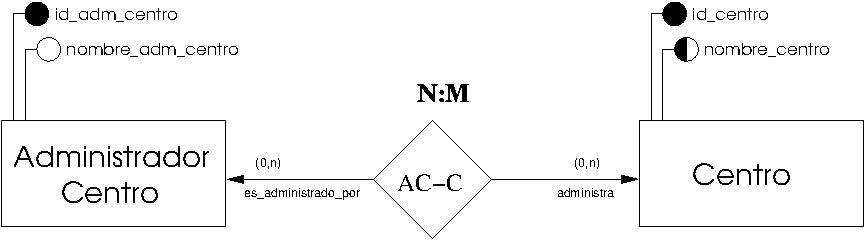
\includegraphics[]{07.Modelo_Entidad-Interrelacion/7.3.Analisis_Interrelaciones/diagramas/AC-C.pdf}
            \caption{Diagrama de la interrelación AC-C.}
            \label{diagramaAC-C}
            \end{center}
         \end{figure}

      \item[Ejemplo práctico del tipo de interrelación]

      \item \begin{center}
            \begin{tabular}{ | c | c | }
            \hline
            \multicolumn{2}{ | c | }{\textbf{Tipo de interrelación AC-C}} \\
            \hline
            \textbf{Administrador Centro} & \textbf{Centro}\\
            \hline
            id\_adm\_centro & id\_centro \\
            \hline
            9 & 15 \\
            \hline
            \end{tabular}
         \end{center}

   \end{description}

\subsection{Interrelación Centro - Titulación}

   \begin{description}
      \item[Definición]

      \item[Características] La interrelación presenta las siguientes
                             características:

         \begin{itemize}
            \item \textbf{Nombre:}
            \item \textbf{Tipo de la interrelación:}
            \item \textbf{Cardinalidad de la interrelación:}
            \item \textbf{Número de atributos:}
         \end{itemize}

      \item[Diagrama] La figura \textit{RELLENAR} muestra el diagrama de la
                      interrelación.

      \item[Descripción de los atributos]

      \item[Ejemplo práctico del tipo de interrelación]
   \end{description}

\subsection{Interrelación Titulación - Asignatura}

   \begin{description}
      \item[Definición] En esta interrelación se deja constancia de que cada
      titulación establecida en el sistema podrá disponer de varias asignaturas.

      \begin{itemize}
       \item Una titulación puede disponer de varias asignaturas.
       \item Una asignatura solamente puede pertenecer a una determinada
             titulación.
      \end{itemize}

      \item[Características] La interrelación presenta las siguientes
                             características:

         \begin{itemize}
            \item \textbf{Nombre:} T-A
            \item \textbf{Tipo de la interrelación:} El tipo de entidad
                  Asignatura es débil por identificación respecto al tipo de
                  entidad Titulación.
            \item \textbf{Cardinalidad de la interrelación:} 1:N
                  \begin{itemize}
                     \item Titulación: dispone\_de (0,n)
                     \item Asignatura: pertenece\_a (1,1)
                  \end{itemize}
            \item \textbf{Número de atributos:} Ninguno.
         \end{itemize}

      \item[Diagrama] La figura \ref{diagramaT-A} muestra el diagrama de la
                      interrelación.

      \item \begin{figure}[!ht]
            \begin{center}
            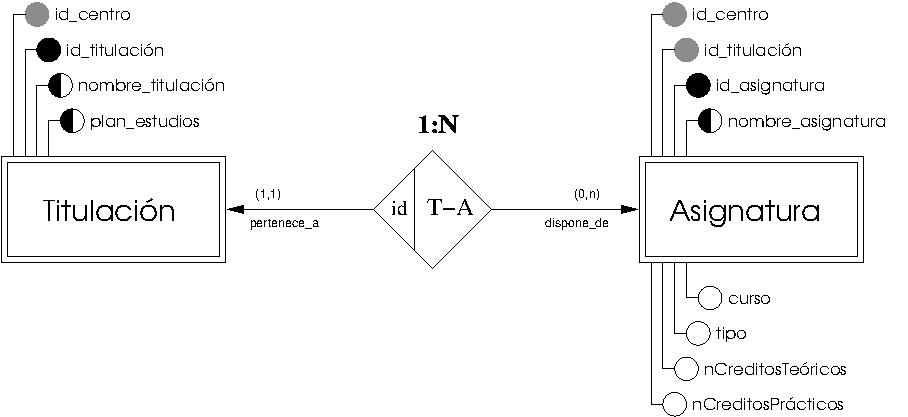
\includegraphics[]{07.Modelo_Entidad-Interrelacion/7.3.Analisis_Interrelaciones/diagramas/T-A.pdf}
            \caption{Diagrama de la interrelación T-A.}
            \label{diagramaT-A}
            \end{center}
         \end{figure}

      \item[Ejemplo práctico del tipo de interrelación]

      \item \begin{center}
            \begin{tabular}{ | r r | }
            \hline
            \multicolumn{2}{ | c | }{\textbf{Tipo de interrelación T-A}} \\
            \hline
            \textbf{Titulación} & \\
            id\_centro & 15 \\
            id\_titulación & 3 \\
            \hline
            \textbf{Asignatura} & \\
            id\_centro & 15 \\
            id\_titulación & 3 \\
            id\_asignatura & 17 \\
            \hline
            \end{tabular}
         \end{center}
   \end{description}

\subsection{Interrelación Asignatura - Asignatura Curso Académico}

   \begin{description}
      \item[Definición]

      \item[Características] La interrelación presenta las siguientes
                             características:

         \begin{itemize}
            \item \textbf{Nombre:}
            \item \textbf{Tipo de la interrelación:}
            \item \textbf{Cardinalidad de la interrelación:}
            \item \textbf{Número de atributos:}
         \end{itemize}

      \item[Diagrama] La figura \textit{RELLENAR} muestra el diagrama de la
                      interrelación.

      \item[Descripción de los atributos]

      \item[Ejemplo práctico del tipo de interrelación]
   \end{description}

\subsection{Interrelación Alumno - Alumno Curso Académico}

   \begin{description}
      \item[Definición] En esta interrelación se deja constancia de que un
      alumno puede estar matriculado durante un número indeterminado de cursos
      académicos.

      \item[Características] La interrelación presenta las siguientes
                             características:

         \begin{itemize}
            \item \textbf{Nombre:} A-AlCA
            \item \textbf{Tipo de la interrelación:} El tipo de entidad
                  Alumno Curso Académico es débil por identificación respecto al
                  tipo de entidad Alumno.
            \item \textbf{Cardinalidad de la interrelación:} 1:N
                  \begin{itemize}
                     \item Alumno: matriculado\_en (0,n)
                     \item Alumno Curso Académico: es\_un (1,1)
                  \end{itemize}
            \item \textbf{Número de atributos:} Ninguno.
         \end{itemize}

      \item[Diagrama] La figura \ref{diagramaA-AlCA} muestra el diagrama de la
                      interrelación.

      \item \begin{figure}[!ht]
            \begin{center}
            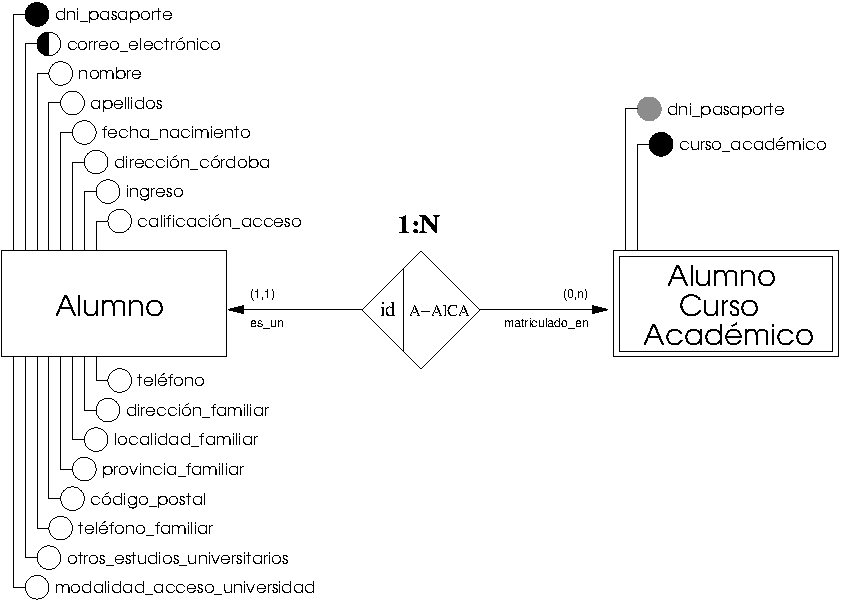
\includegraphics[]{07.Modelo_Entidad-Interrelacion/7.3.Analisis_Interrelaciones/diagramas/A-AlCA.pdf}
            \caption{Diagrama de la interrelación A-AlCA.}
            \label{diagramaA-AlCA}
            \end{center}
         \end{figure}

      \item[Ejemplo práctico del tipo de interrelación]

      \item \begin{center}
            \begin{tabular}{ | r r | }
            \hline
            \multicolumn{2}{ | c | }{\textbf{Tipo de interrelación A-AlCA}} \\
            \hline
            \textbf{Alumno} & \\
            dni\_pasaporte & 01234567A \\
            \hline
            \textbf{Alumno Curso Académico} & \\
            dni\_pasaporte & 01234567A \\
            curso\_académico & 2008 \\
            \hline
            \end{tabular}
         \end{center}
   \end{description}

\subsection{Interrelación Asignatura Curso Académico - Alumno Curso Académico}

   \begin{description}
      \item[Definición] En esta interrelación se deja constancia de que un
      alumno matriculado durante un curso académico está matriculado de un
      determinado de un número indeterminado de asignaturas, las cuales
      pertenecen a un determinado curso académico.

      \item[Características] La interrelación presenta las siguientes
                             características:

         \begin{itemize}
            \item \textbf{Nombre:} ACA-AlCA
            \item \textbf{Tipo de la interrelación:} Fuerte.
            \item \textbf{Cardinalidad de la interrelación:} N:M
            \item \textbf{Número de atributos:} 1, nota.
         \end{itemize}

      \item[Diagrama] La figura \ref{diagramaACA-AlCA} muestra el diagrama de la
                      interrelación.

       \item \begin{figure}[!ht]
            \begin{center}
            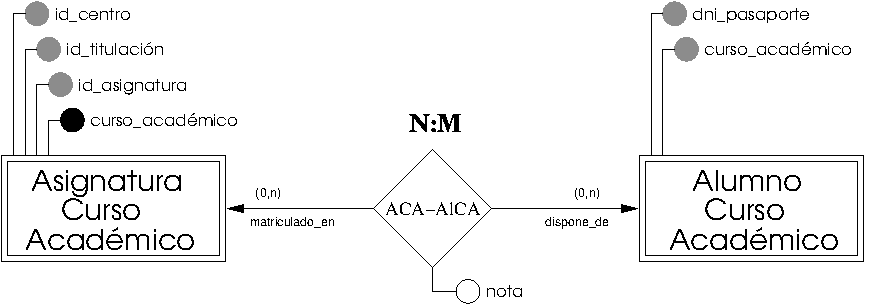
\includegraphics[]{07.Modelo_Entidad-Interrelacion/7.3.Analisis_Interrelaciones/diagramas/ACA-AlCA.pdf}
            \caption{Diagrama de la interrelación ACA-AlCA.}
            \label{diagramaACA-AlCA}
            \end{center}
         \end{figure}

      \item[Descripción de los atributos]

      \item \begin{description}
               \item[Nota] Establece la calificación obtenida por un alumno en
               una asignatura durante un curso académico.
             \end{description}

      \item[Ejemplo práctico del tipo de interrelación]

      \item \begin{center}
            \begin{tabular}{ | r r | }
            \hline
            \multicolumn{2}{ | c | }{\textbf{Tipo de interrelación ACA-AlCA}} \\
            \hline
            \textbf{Asignatura Curso Académico} & \\
            id\_centro & 15 \\
            id\_titulación & 3 \\
            id\_asignatura & 17 \\
            curso\_académico & 2008\\
            \hline
            \textbf{Alumno Curso Académico} & \\
            dni\_pasaporte & 01234567A \\
            curso\_académico & 2008 \\
            \hline
            \textbf{Atributos} & \\
            nota & 7,5 \\
            \hline
            \end{tabular}
         \end{center}
   \end{description}

\subsection{Interrelación Asesor - Asesor Curso Académico}

   \begin{description}
      \item[Definición] En esta interrelación se deja constancia de que un
      asesor puede ofrecer servicios de asesoría durante distintos cursos
      académicos.

      \begin{itemize}
       \item Un \textit{Asesor} puede asesorar a varios \textit{Asesor Curso Académico}.
       \item Un \textit{Asesor Curso Académico} es un \textit{Asesor}.
      \end{itemize}

      \item[Características] La interrelación presenta las siguientes
                             características:

         \begin{itemize}
            \item \textbf{Nombre:} Ase-AseCA
            \item \textbf{Tipo de la interrelación:} El tipo de entidad
                  Asesor Curso Académico es débil por identificación respecto al
                  tipo de entidad Asesor.
            \item \textbf{Cardinalidad de la interrelación:} 1:N
                  \begin{itemize}
                     \item Asesor: asesora (0,n)
                     \item Asesor Curso Académico: es\_un (1,1)
                  \end{itemize}
            \item \textbf{Número de atributos:} Ninguno.
         \end{itemize}

      \item[Diagrama] La figura \ref{diagramaAse-AseCA} muestra el diagrama de la
                      interrelación.

      \item \begin{figure}[!ht]
            \begin{center}
            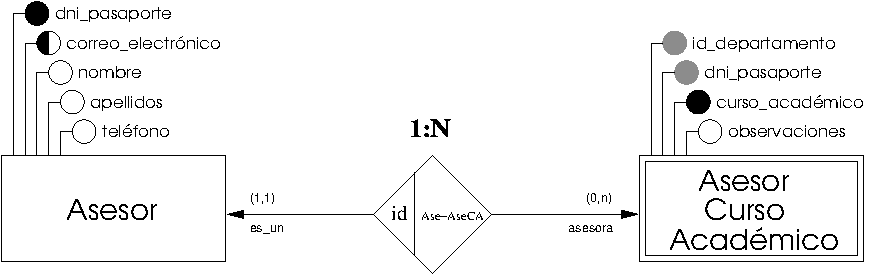
\includegraphics[]{07.Modelo_Entidad-Interrelacion/7.3.Analisis_Interrelaciones/diagramas/Ase-AseCA.pdf}
            \caption{Diagrama de la interrelación Ase-AseCA.}
            \label{diagramaAse-AseCA}
            \end{center}
         \end{figure}

      \item[Ejemplo práctico del tipo de interrelación]

      \item \begin{center}
            \begin{tabular}{ | r r | }
            \hline
            \multicolumn{2}{ | c | }{\textbf{Tipo de interrelación Ase-AseCA}} \\
            \hline
            \textbf{Asesor} & \\
            dni\_pasaporte & 98765432Z \\
            \hline
            \textbf{Asesor Curso Académico} & \\
            dni\_pasaporte & 98765432Z \\
            id\_centro & 2008 \\
            \hline
            \end{tabular}
         \end{center}
   \end{description}

\subsection{Interrelación Departamento - Asesor Curso Académico}

   \begin{description}
      \item[Definición] En esta interrelación se deja constancia de que un
      asesor puede ofrecer servicios de asesoría perteneciendo a un departamento
      durante un determinado curso académico.

      \item[Características] La interrelación presenta las siguientes
                             características:

         \begin{itemize}
            \item \textbf{Nombre:} D-AseCA
            \item \textbf{Tipo de la interrelación:} El tipo de entidad
                  Asesor Curso Académico es débil por existencia respecto al
                  tipo de entidad Departamento.
            \item \textbf{Cardinalidad de la interrelación:} 1:N
            \item \textbf{Número de atributos:} Ninguno.
         \end{itemize}

      \item[Diagrama] La figura \ref{diagramaD-AseCA} muestra el diagrama de la
                      interrelación.

      \item \begin{figure}[!ht]
            \begin{center}
            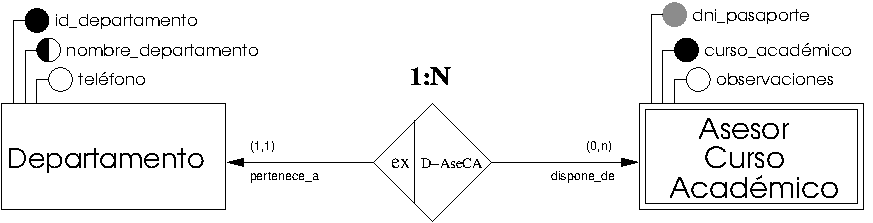
\includegraphics[]{07.Modelo_Entidad-Interrelacion/7.3.Analisis_Interrelaciones/diagramas/D-AseCA.pdf}
            \caption{Diagrama de la interrelación D-AseCA.}
            \label{diagramaD-AseCA}
            \end{center}
         \end{figure}

      \item[Ejemplo práctico del tipo de interrelación]

      \item \begin{center}
            \begin{tabular}{ | r r | }
            \hline
            \multicolumn{2}{ | c | }{\textbf{Tipo de interrelación D-AseCA}} \\
            \hline
            \textbf{Departamento} & \\
            id\_departamento & 22 \\
            \hline
            \textbf{Asesor Curso Académico} & \\
            dni\_pasaporte & 98765432Z \\
            curso\_académico & 2007 \\
            \hline
            \end{tabular}
         \end{center}
   \end{description}

\subsection{Interrelación Asesor Curso Académico - Alumno Curso Académico}

   \begin{description}
      \item[Definición] En esta interrelación se deja constancia de que un
      asesor puede ofrecer servicios de asesoría a un número indeterminado de
      alumnos matriculados durante un determinado curso académico.

      \item[Características] La interrelación presenta las siguientes
                             características:

         \begin{itemize}
            \item \textbf{Nombre:} AseCA-AlCA
            \item \textbf{Tipo de la interrelación:} El tipo de entidad
                  Alumno Curso Académico es débil por existencia respecto al
                  tipo de entidad Asesor Curso Académico.
            \item \textbf{Cardinalidad de la interrelación:} 1:N
                  \begin{itemize}
                     \item Asesor Curso Académico: asesora\_a (0,n)
                     \item Alumno Curso Académico: es\_asesorado\_por (1,1)
                  \end{itemize}
            \item \textbf{Número de atributos:} Ninguno.
            \item \textbf{Restricciones:} Los atributos
                   \textit{curso\_académico} de cada una de las dos entidades
                   que participan en esta interrelación deben tener el mismo
                   valor, por la propia naturaleza de dicha interrelación.
         \end{itemize}

      \item[Diagrama] La figura \ref{diagramaAseCA-AlCA} muestra el diagrama de
                      la interrelación.

       \item \begin{figure}[!ht]
            \begin{center}
            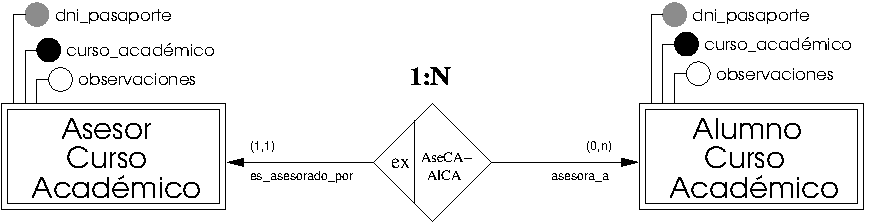
\includegraphics[]{07.Modelo_Entidad-Interrelacion/7.3.Analisis_Interrelaciones/diagramas/AseCA-AlCA.pdf}
            \caption{Diagrama de la interrelación AseCA-AlCA.}
            \label{diagramaAseCA-AlCA}
            \end{center}
         \end{figure}

      \item[Ejemplo práctico del tipo de interrelación]

      \item \begin{center}
            \begin{tabular}{ | r r | }
            \hline
            \multicolumn{2}{ | c | }{\textbf{Tipo de interrelación AseCA-AlCA}} \\
            \hline
            \textbf{Asesor Curso Académico} & \\
            dni\_pasaporte & 98765432Z \\
            curso\_académico & 2008 \\
            \hline
            \textbf{Alumno Curso Académico} & \\
            dni\_pasaporte & 01234567A \\
            curso\_académico & 2008 \\
            \hline
            \end{tabular}
         \end{center}
   \end{description}

\subsection{Interrelación Asesor - Entrevista General}

   \begin{description}
      \item[Definición] En esta interrelación se deja constancia de que un
      asesor puede hacer uso de las entrevistas generales.

      \item[Características] La interrelación presenta las siguientes
                             características:

         \begin{itemize}
            \item \textbf{Nombre:} Ase-EntGen
            \item \textbf{Tipo de la interrelación:} Fuerte.
            \item \textbf{Cardinalidad de la interrelación:} N:M
                  \begin{itemize}
                     \item Asesor: utiliza (0,n)
                     \item Entrevista General: utilizada\_por (0,n)
                  \end{itemize}
            \item \textbf{Número de atributos:} Ninguno.
         \end{itemize}

      \item[Diagrama] La figura \ref{diagramaAse-EntGen} muestra el diagrama de la
                      interrelación.

      \item \begin{figure}[!ht]
            \begin{center}
            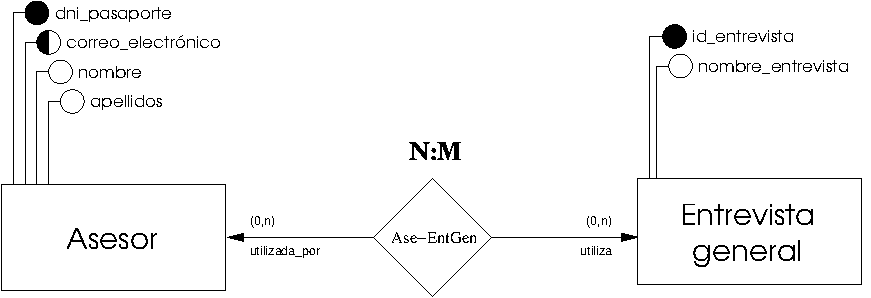
\includegraphics[]{07.Modelo_Entidad-Interrelacion/7.3.Analisis_Interrelaciones/diagramas/Ase-EntGen.pdf}
            \caption{Diagrama de la interrelación Ase-EntGen.}
            \label{diagramaAse-EntGen}
            \end{center}
         \end{figure}

      \item[Ejemplo práctico del tipo de interrelación]

      \item \begin{center}
            \begin{tabular}{ | r r | }
            \hline
            \multicolumn{2}{ | c | }{\textbf{Tipo de interrelación Ase-EntGen}} \\
            \hline
            \textbf{Asesor} & \\
            dni\_pasaporte & 98765432Z \\
            \hline
            \textbf{Entrevista Asesor} & \\
            id\_entrevista & 24 \\
            \hline
            \end{tabular}
         \end{center}
   \end{description}

\subsection{Interrelación Asesor - Entrevista Asesor}

   \begin{description}
      \item[Definición] En esta interrelación se deja constancia de que un
      asesor puede hacer uso de las entrevistas de asesor.

      \item[Características] La interrelación presenta las siguientes
                             características:

         \begin{itemize}
            \item \textbf{Nombre:} Ase-EntAse
            \item \textbf{Tipo de la interrelación:} El tipo de entidad
                  Entrevista Asesor es débil por identificación respecto al
                  tipo de entidad Asesor.
            \item \textbf{Cardinalidad de la interrelación:} 1:N
                  \begin{itemize}
                     \item Asesor: utiliza (0,n)
                     \item Entrevista Asesor: utilizada\_por (1,1)
                  \end{itemize}
            \item \textbf{Número de atributos:} Ninguno.
         \end{itemize}

      \item[Diagrama] La figura \ref{diagramaAse-EntAse} muestra el diagrama de la
                      interrelación.

      \item \begin{figure}[!ht]
            \begin{center}
            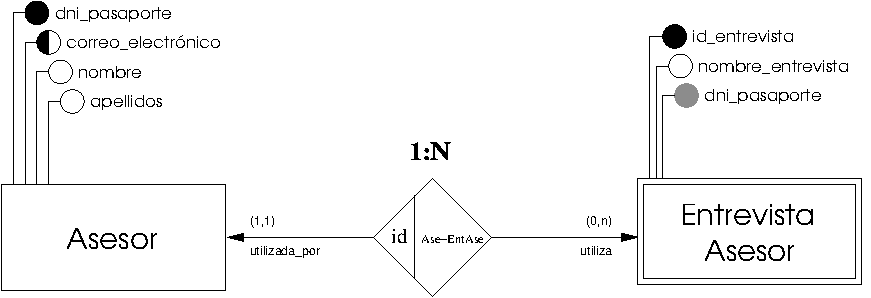
\includegraphics[]{07.Modelo_Entidad-Interrelacion/7.3.Analisis_Interrelaciones/diagramas/Ase-EntAse.pdf}
            \caption{Diagrama de la interrelación Ase-EntAse.}
            \label{diagramaAse-EntAse}
            \end{center}
         \end{figure}

      \item[Ejemplo práctico del tipo de interrelación]

      \item \begin{center}
            \begin{tabular}{ | r r | }
            \hline
            \multicolumn{2}{ | c | }{\textbf{Tipo de interrelación Ase-EntAse}} \\
            \hline
            \textbf{Asesor} & \\
            dni\_pasaporte & 98765432Z \\
            \hline
            \textbf{Entrevista Asesor} & \\
            id\_entrevista & 77 \\
            dni\_pasaporte & 98765432Z \\
            \hline
            \end{tabular}
         \end{center}
   \end{description}

\subsection{Interrelación Pregunta - Alumno Curso Académico}

   \begin{description}
      \item[Definición] En esta interrelación se deja constancia de que un
      determinado alumno recibe preguntas, por parte de su asesor, que deberá
      responder.

      \item[Características] La interrelación presenta las siguientes
                             características:

         \begin{itemize}
            \item \textbf{Nombre:} P-AlCA
            \item \textbf{Tipo de la interrelación:} Fuerte.
            \item \textbf{Cardinalidad de la interrelación:} N:M
                  \begin{itemize}
                     \item Pregunta: formulada\_a (0,n)
                     \item Alumno Curso Académico: recibe (0,n)
                  \end{itemize}
            \item \textbf{Número de atributos:} Tres: tipo, respuesta y fecha.
         \end{itemize}

      \item[Diagrama] La figura \ref{diagramaP-AlCA} muestra el diagrama de la
                      interrelación.

      \item \begin{figure}[!ht]
            \begin{center}
            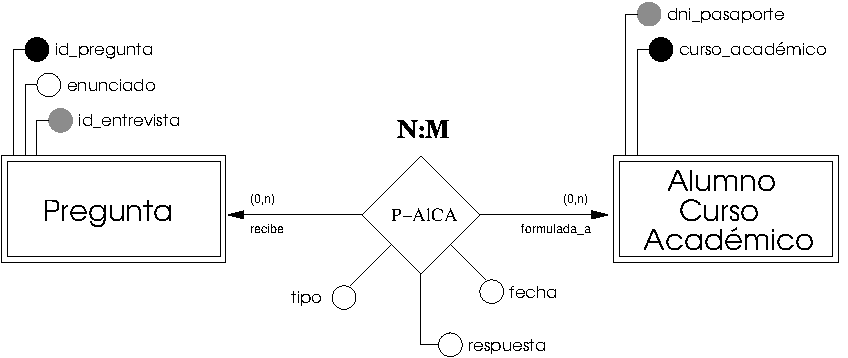
\includegraphics[]{07.Modelo_Entidad-Interrelacion/7.3.Analisis_Interrelaciones/diagramas/P-AlCA.pdf}
            \caption{Diagrama de la interrelación P-AlCA.}
            \label{diagramaP-AlCA}
            \end{center}
         \end{figure}

      \item[Descripción de los atributos] La interrelación presenta los
      siguientes atributos:

       \begin{itemize}
        \item \textbf{tipo}
          \begin{itemize}
            \item \textbf{Definición:} Establece el tipo de pregunta realizada,
            ya sea grupal o individual.
            \item \textbf{Dominio:} Unos de los valores: grupal o individual.
            \item \textbf{Carácter:} Obligatorio.
            \item \textbf{Ejemplo práctico:} individual.
            \item \textbf{Información adicional:} El dato \textbf{¿¿QUIÉN LO INTRODUCE??}.
         \end{itemize}
         \item \textbf{respuesta}
          \begin{itemize}
            \item \textbf{Definición:} Establece la contestación del alumno a la
            pregunta realizada.
            \item \textbf{Dominio:} Conjunto de caracteres alfanuméricos.
            \item \textbf{Carácter:} Obligatorio.
            \item \textbf{Ejemplo práctico:} Alto.
            \item \textbf{Información adicional:} El dato \textbf{¿¿QUIÉN LO INTRODUCE??}.
         \end{itemize}
          \item \textbf{fecha}
          \begin{itemize}
            \item \textbf{Definición:} Establece el día, mes y año cuando se
            formuló la pregunta.
            \item \textbf{Dominio:} Formato de fecha: dd/mm/aaaa.
            \item \textbf{Carácter:} Opcional.
            \item \textbf{Ejemplo práctico:} 01/01/2009.
            \item \textbf{Información adicional:} El dato \textbf{¿¿QUIÉN LO INTRODUCE??}.
         \end{itemize}
       \end{itemize}

      \item[Ejemplo práctico del tipo de interrelación]

      \item \begin{center}
            \begin{tabular}{ | r r | }
            \hline
            \multicolumn{2}{ | c | }{\textbf{Tipo de interrelación P-AlCA}} \\
            \hline
            \textbf{Pregunta} & \\
            id\_pregunta & 36 \\
            enunciado & Nivel de inglés \\
            id\_entrevista & 24 \\
            \hline
            \textbf{Alumno Curso Académico} & \\
            dni\_pasaporte & 01234567A \\
            curso\_académico & 2008 \\
            \hline
            \textbf{Atributos} & \\
            tipo & individual \\
            respuesta & Alto \\
            fecha & 01/01/2009 \\
            \hline
            \end{tabular}
         \end{center}
   \end{description}

